\newpage
\section{Основные теоремы и приложения теории конформных отображений. Теорема Римана, принцип симметрии Римана-Шварца, принцип соответствия границ с обратным принципом соответствия границ.}

\textbf{Основные теоремы и приложения конформных отображения:}\\
\begin{enumerate}
\item \textbf{Теорема Римана} (о возможности конформного и взаимно однозначного отображения одной односвязной области на другую)\\
Пусть $D$ -- односвязная область в $\overline{\mathbb{C}}$, граница которой содержит не менее двух точек. Тогда: 
\begin{enumerate}
    \item $\exists$ голоморфная в $D$ функция $w=f(z)$, которая отображает $D$ конформно и однозначно на единственный круг $G: |w|<1$;
    \item эту функцию можно выбрать так, что $f(z_0)=w_0, \, \textrm{arg} f'(z_0)=\alpha$, где $Z_0 \in D, \, w_0 \in G$ -- заданные точки, $\alpha$ -- заданное действительное число.
\end{enumerate}
Функция $f$, удовлетворяющая 1. и 2. единственная.\\[2mm]

\item \textbf{Принцип симметрии Римана-Шварца}\\
Пусть $D_1$ -- односвязная область, лежащая в верхней полуплоскости $Im z>0$, граница Г$_1$, которая содержит интервал $\gamma$ действительной оси $Im z =0$, область $D_2$ симметрична $D_1$ относительно действительной оси, функция $f(z)$ непрерывна на $D_1$, Г$_1$, голоморфна на $D_1$ и принимает действительные занчения на $\gamma$. Тогда функция $f$ может голоморфно продолжить в область $D_1 \cup \gamma \cup D_2$ по формуле:
\begin{equation}
    f(z) = \begin{cases}
        f_1(z), & \textrm{если} z \in D_1 \cup \gamma, \\
        \overline{f_1(\overline{z})}, & \textrm{если} z \in D_2.
    \end{cases}
\end{equation}

\begin{figure}[h]
    \centering
    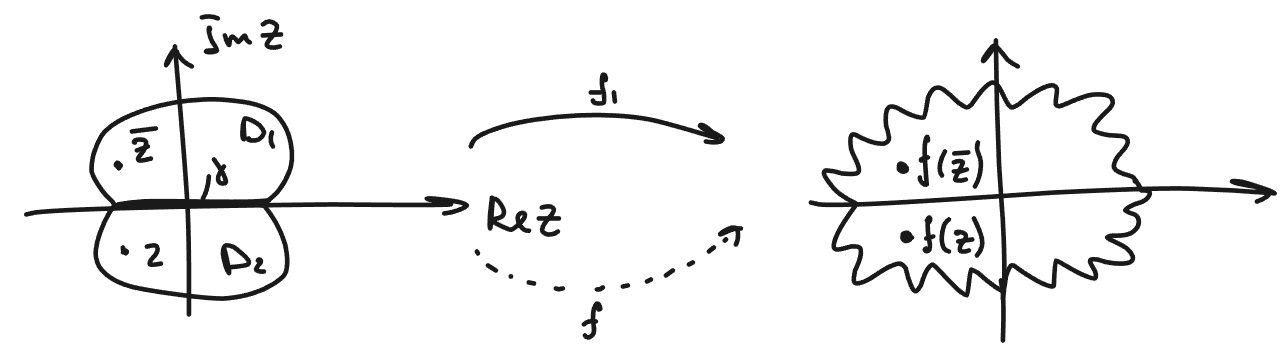
\includegraphics[width=1\linewidth]{answers/img/14_2.png}
\end{figure}

\item \textbf{Принцип соответствия границ}\\
Пусть Г и Г* -- простые контуры, $D$ и $D \ast$ -- односвязные области, ограниченные Г и Г* соответственно, функция $f(z)$ однолистно и конформно отображает $D$ на $D \ast$. Тогда 
\begin{enumerate}
    \item $f(z)$ имеет непрерывное продолжение $\overline{f}$ на Г, то есть $\overline{f}: \overline{D}=D \cup \textrm{Г} \rightarrow \mathbb{C}$ -- непрерывна и $\overline{f}|_D=f$
    \item $\overline{f}$ отображает Г на Г* взаимно однозначно, причемположительному обходу Г соответствует положительный обход Г*.\\[2mm]
\end{enumerate}

\item \textbf{Обратный принцип соответствия границ}\\
Пусть $D$ -- односвязная область в $\mathbb{C}$, ограниченная кусочно-гладким контуром Г. $\overline{D}=D \cup \textrm{Г}, \, f \in H(D),$ функция $f(z)$ отображает контур Г взаимно однозначно на простой кусочно-гладкий контур Г*.\\
Тогда $f(z)$ отображает $D$ конформно и однозначно на область $D \ast$, ограниченную контуром Г*, причем положительному обходу Г соответствует положительный обход Г*.


\end{enumerate}